\documentclass[10pt,twocolumn,a4paper]{article}
\usepackage[margin=2cm]{geometry}
\usepackage[T1]{fontenc}
\usepackage{times}
\usepackage{booktabs,amsmath,amssymb,graphicx,xcolor,url}
\usepackage[hidelinks]{hyperref}
\usepackage{enumitem}
\usepackage{tikz}
\usetikzlibrary{positioning,arrows.meta}
\setlist{nosep,leftmargin=*}
\setlength{\columnsep}{0.6cm}

\title{\textbf{Product Attribute-Value Extraction across Three Eras of NLP:\\CRF, Fine-tuned Transformers, Instruction-tuned LLMs\\and a Cross-Paradigm Evidence-grounded Committee}}
\author{CS F429 Natural Language Processing --- Course Project (Group of 5)\\
\small [Name 1, ID] \quad [Name 2, ID] \quad [Name 3, ID] \quad [Name 4, ID] \quad [Name 5, ID]\\
\small BITS Pilani, Hyderabad Campus}
\date{November 2026}

\begin{document}
\maketitle

\begin{abstract}
Online shops describe products in noisy, unstructured titles and descriptions, while search, faceted navigation and price comparison need structured attribute--value pairs such as \textsc{Brand}=\emph{Xerox} or \textsc{Page Yield}=\emph{25K}. We study attribute-value extraction (AVE) as BIO sequence labelling on two e-commerce benchmarks, WDC-PAVE (1,420 products, 51 attributes) and a reconstructed 5,000-product MAVE pilot (28 attributes), and trace how NLP has evolved on this task: a feature-rich linear-chain CRF (classical), fine-tuned BERT and DeBERTa-v3 (pre-trained Transformers) and Qwen3-4B-Instruct (instruction-tuned LLM) prompted zero-/few-shot with exact evidence verification. As our novel contribution we propose \emph{CPEC}, a cross-paradigm evidence-grounded committee in which models from different eras vote on every candidate span with frequency-band-specific thresholds selected on validation only. On the official WDC-PAVE test set CPEC improves strict entity micro-F1 from 85.77\,$\pm$\,0.40 (DeBERTa, three seeds) to \textbf{86.99\,$\pm$\,0.09}, cutting spurious predictions by 36\% and boundary errors by 43\%. We analyse errors by type, attribute and frequency band, report a negative result on MAVE where only two paradigms are available, and release a reproducible pipeline with a CLI and a GUI demo.
\end{abstract}

\section{Introduction}
Attribute-value extraction takes a product offer (title and description) and returns the values of predefined attributes that are literally mentioned in the text. Figure-style example from WDC-PAVE: from \emph{``435952-B21 HP Xeon E5335 2.0GHz DL360 G5''} we must extract \textsc{Part Number}=\emph{435952-B21}, \textsc{Manufacturer}=\emph{HP}, \textsc{Processor Type}=\emph{Xeon E5335}, \textsc{Clock Speed}=\emph{2.0GHz} and \textsc{Generation}=\emph{G5}. The task is hard because (i)~text is noisy (run-together tokens such as \emph{BlackALTERNATE}, part numbers, units), (ii)~attribute inventories differ per category, (iii)~attribute frequencies are long-tailed, and (iv)~several attributes are easily confused (\textsc{Brand} vs.\ \textsc{Manufacturer}, \textsc{Width} vs.\ \textsc{Height}).

We formulate AVE as BIO sequence labelling \cite{ramshaw1995} and make four contributions: (1)~a controlled comparison of a classical CRF \cite{lafferty2001}, BERT \cite{devlin2019} and DeBERTa-v3 \cite{he2023debertav3} under identical splits, gold data and metrics, with three seeds; (2)~an instruction-tuned LLM study (Qwen3-4B-Instruct \cite{qwen3}) with four prompting conditions, validation-only prompt selection and exact evidence verification against hallucination; (3)~\textbf{CPEC}, a novel cross-paradigm committee that improves over the strongest single model; (4)~detailed quantitative and qualitative error analysis and a working end-to-end demo.

\section{Literature survey}
\textbf{Why the problem matters.} Structured product data drives product search, recommendation, catalogue de-duplication and comparison shopping; most offers on the web, however, carry attributes only in free text \cite{zheng2018opentag,yang2022mave}. Manual curation does not scale to millions of offers and thousands of attributes \cite{xu2019scaling}.

\textbf{Classical approaches.} Early systems used dictionaries, regular expressions and statistical sequence models; CRFs \cite{lafferty2001} with lexical, orthographic and contextual features remained the standard sequence labeller before deep learning.

\textbf{Neural taggers.} OpenTag \cite{zheng2018opentag} combined BiLSTM, CRF and attention for open attribute tagging; SU-OpenTag \cite{xu2019scaling} conditioned on the attribute to scale to thousands of attributes; AVEQA \cite{wang2020aveqa} cast AVE as question answering with BERT. Pre-trained Transformers \cite{devlin2019,he2021deberta,he2023debertav3} are now the default strong baselines.

\textbf{Datasets.} MAVE \cite{yang2022mave} provides 2.2M Amazon products with 3M attribute annotations across 1,257 categories; WDC-PAVE \cite{brinkmann2024wdcpave} offers 1,420 web shop offers from five categories and is designed to test generalisation to heterogeneous web data.

\textbf{LLMs.} Instruction-tuned LLMs can extract attributes zero-/few-shot \cite{brown2020,brinkmann2024extractgpt}, removing the need for large labelled sets, but they may produce values that are not in the text (hallucination \cite{ji2023hallucination}), vary their surface form and are costly at inference time. Combining heterogeneous models is a classical way to reduce variance and correct independent errors \cite{dietterich2000}; our committee applies this idea \emph{across paradigms} and grounds the LLM's votes in the input text.

\section{Datasets}
\textbf{WDC-PAVE} \cite{brinkmann2024wdcpave} (domain: e-commerce web offers from many shops; source: Web Data Commons). We use the official 354-product test set and split the remaining 1,066 products into 906 train / 160 validation products, grouping by product cluster so that offers of the same real-world product never cross splits. Categories: Computers \& Accessories, Home \& Garden, Office Products, Jewelry, Grocery \& Gourmet Food. Each attribute value records whether it occurs in the title, the description or both.

\textbf{MAVE pilot} (domain: Amazon product pages). Because MAVE releases only labels, product text must be re-joined with the Amazon Review 2018 metadata. We reconstructed a frozen 5,000-product pilot from the five largest categories (Shoes, Shirts \& Tops, Watches, Books, Dresses): 3,548 / 736 / 716 train / validation / test products, split by connected duplicate groups (identical cleaned text or shared parent ASIN), with 28 predefined attributes (57 BIO labels; 25 occur in training). All files are hashed; the selection manifest is in \texttt{datasets/mave\_pilot/}.

\begin{table}[t]\centering\small
\begin{tabular}{lrrr}\toprule
WDC-PAVE & Train & Val & Test \\\midrule
Products & 906 & 160 & 354 \\
Sequences (title/descr.) & 1,812 & 320 & 708 \\
Tokens & 64,962 & 11,536 & 24,952 \\
Entity spans & 8,810 & 1,596 & 3,418 \\
Attributes present & 51 & 50 & 51 \\
Values not found in text & 40 & 7 & 16 \\
Overlapping annotations dropped & 120 & 15 & 62 \\\midrule
MAVE pilot products & 3,548 & 736 & 716 \\
MAVE sequences & 43,302 & -- & -- \\\bottomrule
\end{tabular}
\caption{Dataset statistics after preprocessing.}\label{tab:data}
\end{table}

\textbf{Preprocessing.} Gold values are matched case-insensitively in their recorded source; if a value occurs more than once we label one occurrence (values with fewer matches and longer values are placed first; the first non-overlapping occurrence wins); overlapping annotations are rejected and logged; ``n/a'' values are skipped. Text is tokenised with \verb|\w+([./'’-]\w+)*| or single punctuation, and gold span edges are forced to be token boundaries (e.g.\ \emph{BlackALTERNATE}$\rightarrow$\emph{Black}+\emph{ALTERNATE}). Attribute names are normalised (\emph{Color(s)}$\rightarrow$\textsc{Color\_S}). No stemming or stop-word removal is applied: casing, digits and punctuation carry the attribute signal (part numbers, units). Our cleaned re-implementation reproduces the Phase~2 files exactly (all 320 validation and 708 test sequences identical).

\textbf{Limitations.} (i)~\emph{Imbalance}: 21 head attributes ($>$100 training spans) carry 85\% of test spans, while 8 tail attributes have 5--19 spans. (ii)~\emph{Category bias}: Computers and Home \& Garden dominate WDC-PAVE; MAVE is fashion/book heavy. (iii)~\emph{Annotation}: only one occurrence per value is labelled, repeated mentions are unlabelled, and MAVE annotations are incomplete (unannotated attributes are unknown, not absent). (iv)~Gold-assisted boundaries make benchmark tokenisation slightly optimistic; our demo uses an annotation-free tokenizer. (v)~The MAVE pilot is not the official full MAVE benchmark.

\section{Methods}
\begin{figure*}[t]\centering\small
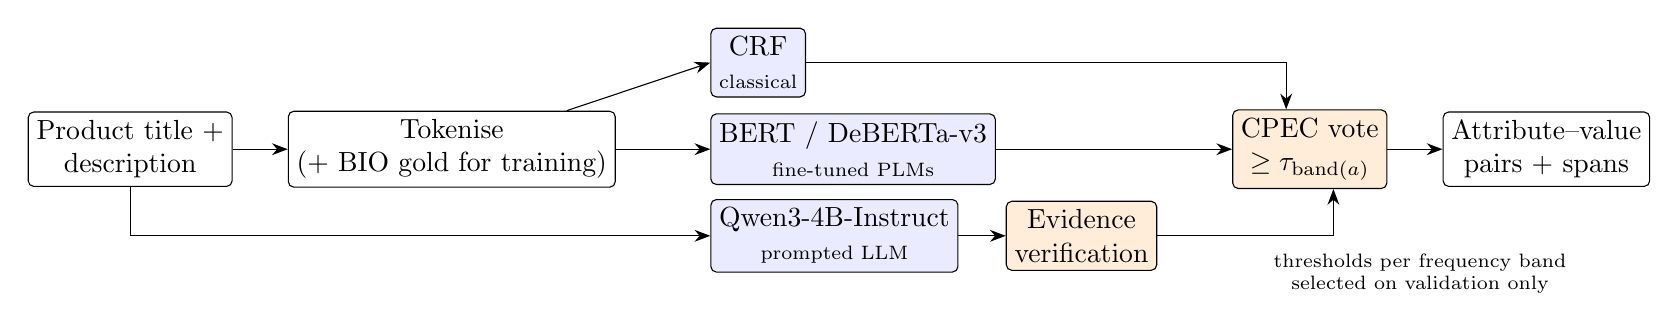
\begin{tikzpicture}[node distance=4mm and 7mm, box/.style={draw, rounded corners=2pt, align=center, minimum height=8mm, inner sep=3pt, fill=#1}, box/.default=white, >={Stealth[length=2mm]}]
\node[box] (in) {Product title +\\description};
\node[box, right=of in] (tok) {Tokenise\\(+ BIO gold for training)};
\node[box=blue!8, right=12mm of tok, yshift=11mm] (crf) {CRF\\\scriptsize classical};
\node[box=blue!8, right=12mm of tok] (bert) {BERT / DeBERTa-v3\\\scriptsize fine-tuned PLMs};
\node[box=blue!8, right=12mm of tok, yshift=-11mm] (llm) {Qwen3-4B-Instruct\\\scriptsize prompted LLM};
\node[box=orange!15, right=6mm of llm] (ev) {Evidence\\verification};
\node[box=orange!15, right=30mm of bert] (vote) {CPEC vote\\$\ge\tau_{\mathrm{band}(a)}$};
\node[box, right=of vote] (out) {Attribute--value\\pairs + spans};
\draw[->] (in) -- (tok); \draw[->] (tok) -- (crf.west); \draw[->] (tok) -- (bert); \draw[->] (in.south) |- (llm.west);
\draw[->] (crf.east) -| ([xshift=-3mm]vote.north) ; \draw[->] (bert) -- (vote); \draw[->] (llm) -- (ev); \draw[->] (ev.east) -| ([xshift=3mm]vote.south);
\draw[->] (vote) -- (out);
\node[below=1mm of vote, font=\scriptsize, align=center, xshift=14mm, yshift=-6mm] {thresholds per frequency band\\selected on validation only};
\end{tikzpicture}
\caption{System overview. Models from three eras of NLP extract candidates; the LLM's values must pass exact evidence verification; the cross-paradigm committee (CPEC) keeps candidates with enough votes, using frequency-band-specific thresholds chosen on validation.}\label{fig:system}
\end{figure*}

\subsection{Classical baseline: CRF}
A linear-chain CRF \cite{lafferty2001} (CRFsuite \cite{okazaki2007} via sklearn-crfsuite) with features for the current token (lower-cased word, 1--3 character prefixes and suffixes, upper/lower/title/digit flags, presence of digits, letters, \texttt{-}, \texttt{/}, \texttt{.}, \texttt{\%}, word shape such as \emph{2.4GHz}$\rightarrow$\emph{d.dXxx}, source field) and the same lexical/shape features of the previous and next token. Training: L-BFGS, $c_1{=}0.1$ (L1), $c_2{=}0.1$ (L2), 150 iterations, all possible transitions; $c_1,c_2$ chosen by grid search on validation.

\subsection{Pre-trained Transformers: BERT and DeBERTa-v3}
\textbf{Architecture.} Encoder + dropout + linear layer over the $2K{+}1$ BIO labels (103 labels on WDC). \texttt{bert-base-uncased}: 12 layers, hidden size 768, 12 attention heads, WordPiece (30k), absolute position embeddings, 110M parameters. \texttt{deberta-v3-base}: 12 layers, 768 hidden, 12 heads, disentangled content/relative-position attention, SentencePiece vocabulary of 128k, ELECTRA-style replaced-token-detection pre-training \cite{he2021deberta,he2023debertav3}, 184M parameters. Both checkpoints are pinned to a Hugging Face revision.

\textbf{Fine-tuning.} All weights are updated (no frozen embeddings). Only the first sub-word of each word is supervised (other sub-words have label $-100$); a word's prediction is the arg-max of its first sub-word. AdamW, learning rate $5\cdot10^{-5}$ (selected from $\{1,2,5\}\cdot10^{-5}$ on validation), weight decay 0.01 (not on bias/LayerNorm), batch 16, linear decay without warm-up, gradient clipping 1.0, maximum length 512 sub-words with no truncation, bf16 autocast. Development runs allowed 15 epochs with early-stopping patience 3. Final models are retrained on train+validation for a fixed budget equal to the median best development epoch (BERT 14, DeBERTa 15 on WDC; DeBERTa 10 on MAVE) and evaluated once on test for seeds 42/43/44. Implementation: PyTorch, Hugging Face Transformers \cite{wolf2020}; HPC GPU node (SLURM).

\subsection{Instruction-tuned LLM: Qwen3-4B-Instruct}
\texttt{Qwen/Qwen3-4B-Instruct-2507} \cite{qwen3} (4B parameters, 36 layers, grouped-query attention, revision pinned) is used without fine-tuning. The system prompt asks for a JSON object \verb|{"attributes":[{attribute,value,source}]}| with values copied verbatim, no normalisation or inference, and states that product text is untrusted data. Four controlled conditions are run on the same 49 stratified validation products: \emph{zero-shot} (global attribute list), \emph{schema-guided} (category-specific attributes with short definitions, e.g.\ ``\textsc{Brand}: brand explicitly identifying the offered product, not a compatibility target''), \emph{one-shot} and \emph{three-shot} (training products of the same category as demonstrations). Greedy decoding, at most 768 new tokens, 12,288-token context, no truncation. \textbf{Evidence verification}: a predicted value is kept only if it occurs literally in the product text (otherwise it is counted as an unsupported/hallucinated value). The prompt with the best verified validation F1 is frozen and run on all 354 test products. Hardware: Kaggle 2$\times$T4 (fp16) or an Apple-Silicon Mac (MPS).

\subsection{Novel contribution: Cross-Paradigm Evidence-grounded Committee (CPEC)}
\textbf{Observation.} Phase~2 error analysis showed that the three model families fail differently. The CRF is precise but misses values (val P\,83.4 / R\,74.9). DeBERTa has high recall but over-generates: 212 spurious, 199 boundary-shifted and 155 wrongly-typed spans on the WDC test set. Errors of models trained in different paradigms (hand-crafted features, pre-trained contextual encoders, prompted LLMs) are therefore only partly correlated, which is exactly the situation in which voting helps \cite{dietterich2000}.

\textbf{Method.} For a sentence, each voter $m$ (CRF, BERT, DeBERTa, and optionally the LLM) contributes its set of predicted spans $(a, i, j)$ (attribute, start, end). A candidate is kept iff
\[\textstyle\sum_m w_m\,[\,(a,i,j)\in S_m\,] \;\ge\; \tau_{\,\mathrm{band}(a)},\]
where $\mathrm{band}(a)\in$\{head, medium, tail, extreme tail\} is determined by the attribute's training span count ($>$100, 20--100, 5--19, $<$5) and $w_m{=}1$. Overlapping survivors are resolved in favour of the span with more votes. When the LLM participates, voting is done on product-level (attribute, value) pairs, and the LLM may vote only for values that passed evidence verification, so it can never inject a hallucinated value.

\textbf{Selection.} The thresholds $\tau$ are chosen by exhaustive grid search ($\tau\in\{1,\dots,M\}$ per band) on the \emph{validation} split, maximising the mean micro-F1 over the three seed-matched voter groups (ties favour lower thresholds, i.e.\ higher recall). They are frozen before scoring test. CPEC needs no extra training and adds negligible inference cost to the base models.

\textbf{What is new.} Figure~\ref{fig:system} gives an overview. Instead of ensembling several runs of one architecture, CPEC deliberately mixes models from different eras of NLP and makes the vote attribute-frequency aware; for the LLM it replaces trust in generated text with literal evidence. It addresses the assumption that the newest single model is the best extractor, and targets the dominant precision errors of fine-tuned Transformers.


\begin{table}[t]\centering\small
\begin{tabular}{lll}\toprule
Model & Key hyper-parameters & Selected on \\\midrule
CRF & L-BFGS, $c_1{=}0.1$, $c_2{=}0.1$, 150 it. & val grid \\
BERT-base & lr $5\mathrm{e}{-5}$, bs 16, 14 ep., wd 0.01 & val LR/epochs \\
DeBERTa-v3-base & lr $5\mathrm{e}{-5}$, bs 16, 15 ep., wd 0.01 & val LR/epochs \\
Qwen3-4B-Instr. & greedy, 768 new tok., 12k ctx & val prompt \\
CPEC & $\tau$ per band $\in\{1..M\}$, $w_m{=}1$ & val grid \\\bottomrule
\end{tabular}
\caption{Hyper-parameters. ep.\ = epochs on train+val for final models; MAVE DeBERTa uses 10 epochs.}\label{tab:hp}
\end{table}
\section{Experiments}
\subsection{Set-up}
All models use the same frozen splits, BIO gold, label inventory and evaluation code; dataset files are verified by SHA-256 before every run. Validation is used for every choice (CRF regularisation, learning rate, epoch budget, prompt, CPEC thresholds); test sets were scored once per frozen configuration. Transformer results are reported for three seeds (mean $\pm$ sample SD).

\subsection{Metrics}
\textbf{Strict entity micro-F1} (seqeval \cite{nakayama2018}): a predicted span counts only if attribute and both boundaries match exactly; this is the standard metric for BIO extraction and penalises partial values such as \emph{Tray} for \emph{Regal Tray}. \textbf{Macro-F1} averages per-attribute F1 and therefore exposes performance on rare attributes. \textbf{Product pair F1}: precision/recall over distinct exact (attribute, value) pairs per product; this is the natural metric for the LLM, which outputs pairs, and reflects what a catalogue actually receives. We also report \textbf{unsupported-value rate} (hallucination) and JSON validity for the LLM. \emph{Limitations}: exact matching gives no credit for semantically equivalent variants (\emph{2.0GHz} vs.\ \emph{2 GHz}); micro-F1 is dominated by head attributes; one-occurrence gold makes repeated correct mentions count as false positives in the span metric.

\subsection{Baselines: classical vs.\ modern}
Table~\ref{tab:cpec_wdc} and Figure~\ref{fig:evo} show the evolution on WDC-PAVE test: CRF 79.34 $\rightarrow$ BERT 83.15 $\rightarrow$ DeBERTa-v3 85.77. Pre-trained encoders mainly gain recall (75.1$\rightarrow$87.2) because contextual sub-word representations generalise to unseen brands and identifiers, while precision stays similar (CRF 84.1, DeBERTa 84.4) or drops (BERT 81.3). DeBERTa's disentangled relative-position attention and larger, case-preserving vocabulary give +2.6 points over the uncased BERT. On MAVE (Table~\ref{tab:cpec_mave}) DeBERTa beats the CRF by 3.2 points (83.97 vs.\ 80.81), again through recall.


\begin{figure}[t]\centering
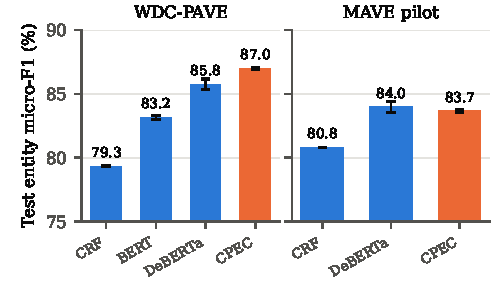
\includegraphics[width=\linewidth]{figures/f1_evolution.pdf}
\caption{Test micro-F1 across the eras of NLP and for CPEC (error bars: SD over three seeds).}\label{fig:evo}
\end{figure}
\begin{table}[t]\centering\small
\begin{tabular}{llrrrr}\toprule
Split & System & P & R & micro-F1 & SD \\\midrule
Val & DeBERTa & 82.55 & 86.42 & 84.44 & 0.40 \\
Val & CRF & 83.40 & 74.94 & 78.94 & -- \\
Val & BERT & 78.69 & 82.60 & 80.60 & 0.60 \\
Val & \textbf{CPEC (ours)} & 87.54 & 82.56 & \textbf{84.98} & 0.52 \\
\midrule
Test & DeBERTa & 84.36 & 87.23 & 85.77 & 0.40 \\
Test & CRF & 84.08 & 75.10 & 79.34 & -- \\
Test & BERT & 81.28 & 85.11 & 83.15 & 0.18 \\
Test & \textbf{CPEC (ours)} & 89.30 & 84.81 & \textbf{86.99} & 0.09 \\
\bottomrule\end{tabular}
\caption{WDC-PAVE entity-level results (strict span micro-F1, \%). Mean over seeds 42/43/44 (CRF is a single model). Vote thresholds selected on validation: head=2, medium=2, tail=2, extreme tail=3.}\label{tab:cpec_wdc}\end{table}

\begin{table}[t]\centering\small
\begin{tabular}{llrrrr}\toprule
Split & System & P & R & micro-F1 & SD \\\midrule
Val & DeBERTa & 78.01 & 87.84 & 82.62 & 0.47 \\
Val & CRF & 80.13 & 80.92 & 80.53 & -- \\
Val & \textbf{CPEC (ours)} & 75.98 & 90.89 & \textbf{82.76} & 0.45 \\
\midrule
Test & DeBERTa & 80.17 & 88.16 & 83.97 & 0.44 \\
Test & CRF & 81.23 & 80.40 & 80.81 & -- \\
Test & \textbf{CPEC (ours)} & 77.77 & 90.52 & \textbf{83.66} & 0.12 \\
\bottomrule\end{tabular}
\caption{MAVE pilot entity-level results. Only two paradigms (CRF, DeBERTa) are available as voters. Mean over seeds 42/43/44 (CRF is a single model). Vote thresholds selected on validation: head=1, medium=1, tail=1, extreme tail=1.}\label{tab:cpec_mave}\end{table}


\subsection{Results of the novel method}
\textbf{WDC-PAVE.} The validation grid selected a majority vote for head, medium and tail attributes (extreme-tail attributes do not occur in WDC). On test, CPEC reaches \textbf{86.99\,$\pm$\,0.09} micro-F1, +1.22 points over DeBERTa (85.77\,$\pm$\,0.40), with every seed improving (+1.49, +0.82, +1.36) and a four-times smaller seed variance. Precision rises from 84.4 to 89.3 while recall drops from 87.2 to 84.8. The same committee evaluated at the product pair level improves DeBERTa from 85.16 to 86.65 F1. A paired bootstrap over test products (2,000 resamples, title and description kept together) confirms the gain for every seed: $\Delta$F1 = +1.49 (95\% CI [0.72, 2.23]), +0.82 ([0.16, 1.52]) and +1.36 ([0.64, 2.12]) points, all $p<0.01$.

\begin{table}[t]\centering\small
\begin{tabular}{llrrrrr}\toprule
Data & System & Correct & Spurious & Boundary & Wrong attr. & Missed \\\midrule
WDC & DeBERTa & 2978 & 212 & 199 & 155 & 147 \\
WDC & CPEC & 2898 & 135 & 114 & 94 & 321 \\
MAVE & DeBERTa & 1382 & 280 & 33 & 29 & 144 \\
MAVE & CPEC & 1427 & 348 & 25 & 29 & 104 \\
\bottomrule\end{tabular}
\caption{Span-level error profile on the test sets (seed 42). Boundary = overlapping span with the right attribute but wrong extent.}\label{tab:errors}\end{table}

\begin{table}[t]\centering\small
\begin{tabular}{lrrr}\toprule
Frequency band & Test spans & DeBERTa & CPEC \\\midrule
head & 2910 & 86.16 & 87.50 \\
medium & 448 & 83.35 & 85.42 \\
tail & 60 & 73.02 & 76.11 \\
\bottomrule\end{tabular}
\caption{WDC-PAVE test micro-F1 by training-frequency band of the attribute (head $>$100 training spans, medium 20--100, tail 5--19), seed 42.}\label{tab:bands}\end{table}

\begin{figure}[t]\centering
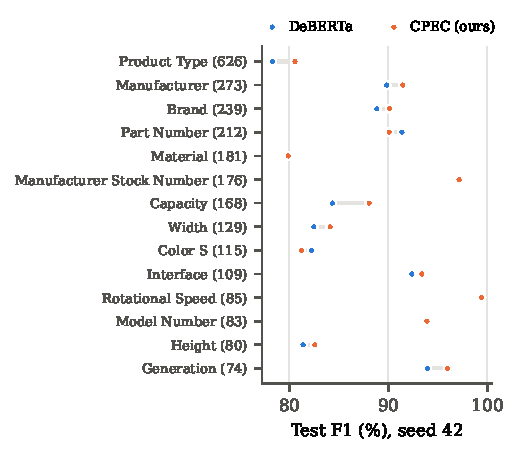
\includegraphics[width=\linewidth]{figures/per_attribute.pdf}
\caption{Per-attribute test F1 for the 14 most frequent WDC-PAVE attributes (test support in brackets). CPEC helps most on \textsc{Capacity}, \textsc{Product Type} and \textsc{Generation}; it slightly hurts \textsc{Part Number} and \textsc{Color(s)}, where the CRF/BERT votes miss valid DeBERTa spans.}\label{fig:attr}
\end{figure}


\textbf{Where the gain comes from} (Table~\ref{tab:errors}). CPEC removes 36\% of spurious spans (212$\rightarrow$135), 43\% of boundary errors (199$\rightarrow$114) and 39\% of wrong-attribute errors (155$\rightarrow$94) at the cost of 174 additional misses. Gains hold in every frequency band (Table~\ref{tab:bands}) and for most frequent attributes (Figure~\ref{fig:attr}), and are largest for medium (+2.1) and tail attributes (+3.1), where single models are least reliable.

\textbf{MAVE: a negative result.} With only two paradigms (no BERT was trained on MAVE) a vote cannot break ties: validation selects the union ($\tau{=}1$), which raises recall to 90.5 but lowers precision, giving 83.66 vs.\ 83.97 for DeBERTa on test; intersection is worse (81.18). This supports our hypothesis that CPEC needs at least three \emph{different} voters and motivates the LLM as the third voter on MAVE.

\textbf{A second negative result.} A first design that routed each frequency band to DeBERTa, CRF, their union or intersection (selected on validation) improved validation only marginally (84.44$\rightarrow$84.49) and lowered test F1 (85.77$\rightarrow$85.60); we therefore moved to the three-voter committee.

\subsection{LLM study}
% LLM results not yet available
\begin{table}[t]\centering\small\fbox{\parbox{0.9\linewidth}{\centering Qwen3-4B results: run \texttt{notebooks/01\_phase3\_qwen\_llm\_wdc.ipynb} (or \texttt{scripts/phase3\_llm/run\_local.py}) and \texttt{scripts/make\_report\_tables.py}.}}\caption{LLM prompting study (pending).}\label{tab:llm}\end{table}

% CPEC+LLM table appears after run_committee_with_llm.py

Table~\ref{tab:llm} reports the four prompting conditions on the same 49 validation products and the selected prompt on all 354 test products, compared with the saved CRF/BERT/DeBERTa predictions under the identical pair metric. Evidence verification can only remove predictions, so it raises (or keeps) precision; the unsupported-value rate measures how often the LLM produced text that is not in the input. Table~\ref{tab:cpecllm} adds the LLM as a fourth, evidence-grounded voter in CPEC.

\subsection{Qualitative error analysis}
Recurring failure patterns (validation, DeBERTa, pair level): (1)~\emph{Granularity}: \emph{Tray} vs.\ gold \emph{Regal Tray}; \emph{24} vs.\ \emph{24 index sets} (\textsc{Pack Quantity}). (2)~\emph{Near-synonymous attributes}: \emph{Safco}, \emph{Waterford} labelled \textsc{Brand} where gold says \textsc{Manufacturer}. (3)~\emph{Axis ambiguity}: \emph{5 7/10} predicted as \textsc{Height} instead of \textsc{Width}; \emph{8-1/2"} as \textsc{Width} instead of \textsc{Length}. (4)~\emph{Unannotated repeated or plausible values}: \emph{white}, \emph{yellow} as \textsc{Color(s)} in descriptions where gold annotated only one mention; arguably annotation gaps. (5)~\emph{Domain jargon}: \emph{s/s} (stainless steel) as \textsc{Material} missed. Mitigations: attribute-specific normalisation and alias lists, schema definitions that disambiguate axes (used in our schema-guided prompts), label-aware decoding that forbids illegal BIO transitions, and annotation of all mentions.

\section{Challenges and how we addressed them}
\begin{itemize}
\item \textbf{Noisy text and value matching}: run-together tokens and values occurring several times. \emph{Solution}: boundary-forcing tokenisation, deterministic one-occurrence selection, logging of 63 unmatched values and 197 overlapping annotations.
\item \textbf{BERT initially underperformed the CRF} (63\% val F1 after 5 epochs). \emph{Solution}: audited alignment, padding masks and metrics, then a bounded learning-rate/epoch study: 80.6\% at lr $5\cdot10^{-5}$ and up to 15 epochs.
\item \textbf{DeBERTa tokenizer differences} (SentencePiece vs.\ WordPiece). \emph{Solution}: separate first-sub-word alignment audit and native/fast tokenizer equivalence check; model revisions pinned.
\item \textbf{MAVE releases labels only}; the 12\,GB Amazon metadata was gzip-compressed twice, which broke the first reconstruction. \emph{Solution}: nested-gzip reader with CRC checks, SHA-256 manifests and a frozen 5,000-product pilot with group-aware splits.
\item \textbf{Test-set discipline}: avoiding selection on test. \emph{Solution}: all choices on validation; final epoch budgets fixed from development runs; CPEC thresholds and LLM prompt frozen before test.
\item \textbf{LLM hallucination and format errors}. \emph{Solution}: strict JSON parsing, schema checks, exact evidence verification; LLM votes count only when grounded.
\item \textbf{Compute}: the HPC allocation ended; the 4B-parameter LLM needs $\sim$8\,GB of weights. \emph{Solution}: portable runner for Kaggle T4 GPUs (model sharding across two GPUs, fp16) and Apple-Silicon MPS, with resumable per-product checkpoints.
\item \textbf{Negative results}: a frequency-routed two-model hybrid and the two-voter MAVE committee did not help; we report them and explain why three different voters are needed.
\end{itemize}

\section{Conclusion}
On product attribute-value extraction, pre-trained Transformers clearly surpass a strong feature-based CRF (+6.4 F1 on WDC-PAVE with DeBERTa-v3), mainly through recall. Their remaining errors are dominated by spurious, boundary and attribute-confusion errors, which models from other paradigms do not share. Our cross-paradigm committee CPEC exploits this and improves the best single model to 86.99 F1 with much lower variance, without any extra training. Future work: attribute-aware value normalisation (units, decimal vs.\ binary capacities), learning voter weights per attribute, and evaluating on the full official MAVE benchmark.

\paragraph{Reproducibility.} Code, data, predictions and this report: \url{https://github.com/REPLACE_WITH_YOUR_USERNAME/nlp-product-attribute-extraction}. \texttt{scripts/phase3\_committee/run\_committee.py} reproduces all entity-level tables from the saved predictions on a CPU in about one minute.

\small
\begin{thebibliography}{99}
\bibitem{brinkmann2024wdcpave} A.~Brinkmann, N.~Baumann, C.~Bizer. 2024. Using LLMs for the Extraction and Normalization of Product Attribute Values. \emph{ADBIS 2024}.
\bibitem{brinkmann2024extractgpt} A.~Brinkmann, R.~Shraga, C.~Bizer. 2024. ExtractGPT: Exploring the Potential of Large Language Models for Product Attribute Value Extraction. \emph{arXiv:2310.12537}.
\bibitem{brown2020} T.~Brown et~al. 2020. Language Models are Few-Shot Learners. \emph{NeurIPS}.
\bibitem{devlin2019} J.~Devlin, M.-W.~Chang, K.~Lee, K.~Toutanova. 2019. BERT: Pre-training of Deep Bidirectional Transformers for Language Understanding. \emph{NAACL}.
\bibitem{dietterich2000} T.~G.~Dietterich. 2000. Ensemble Methods in Machine Learning. \emph{Multiple Classifier Systems}, LNCS 1857.
\bibitem{he2021deberta} P.~He, X.~Liu, J.~Gao, W.~Chen. 2021. DeBERTa: Decoding-enhanced BERT with Disentangled Attention. \emph{ICLR}.
\bibitem{he2023debertav3} P.~He, J.~Gao, W.~Chen. 2023. DeBERTaV3: Improving DeBERTa using ELECTRA-Style Pre-Training with Gradient-Disentangled Embedding Sharing. \emph{ICLR}.
\bibitem{ji2023hallucination} Z.~Ji et~al. 2023. Survey of Hallucination in Natural Language Generation. \emph{ACM Computing Surveys} 55(12).
\bibitem{lafferty2001} J.~Lafferty, A.~McCallum, F.~Pereira. 2001. Conditional Random Fields: Probabilistic Models for Segmenting and Labeling Sequence Data. \emph{ICML}.
\bibitem{nakayama2018} H.~Nakayama. 2018. seqeval: A Python framework for sequence labeling evaluation. \url{https://github.com/chakki-works/seqeval}.
\bibitem{okazaki2007} N.~Okazaki. 2007. CRFsuite: a fast implementation of Conditional Random Fields.
\bibitem{qwen3} Qwen Team. 2025. Qwen3 Technical Report. \emph{arXiv:2505.09388}.
\bibitem{ramshaw1995} L.~Ramshaw, M.~Marcus. 1995. Text Chunking using Transformation-Based Learning. \emph{3rd Workshop on Very Large Corpora}.
\bibitem{wang2020aveqa} Q.~Wang et~al. 2020. Learning to Extract Attribute Value from Product via Question Answering: A Multi-task Approach. \emph{KDD}.
\bibitem{wolf2020} T.~Wolf et~al. 2020. Transformers: State-of-the-Art Natural Language Processing. \emph{EMNLP: System Demonstrations}.
\bibitem{xu2019scaling} H.~Xu, W.~Wang, X.~Mao, X.~Jiang, M.~Lan. 2019. Scaling up Open Tagging from Tens to Thousands: Comprehension Empowered Attribute Value Extraction from Product Title. \emph{ACL}.
\bibitem{yang2022mave} L.~Yang et~al. 2022. MAVE: A Product Dataset for Multi-source Attribute Value Extraction. \emph{WSDM}.
\bibitem{zheng2018opentag} G.~Zheng, S.~Mukherjee, X.~L.~Dong, F.~Li. 2018. OpenTag: Open Attribute Value Extraction from Product Profiles. \emph{KDD}.
\end{thebibliography}
\end{document}
